
\newpage
\section{Merge}

This method is useful to update the release branch of Sofa. The most easily way to do is, is using SVN Tortoise, only available on Windows OS. This tool provides a friendly-user graphic interface to perform the different tasks. 
\begin{itemize}
        \item Open a merge dialog window by a right click in the explorer.
        \begin{figure}[htpb]
	\centering
		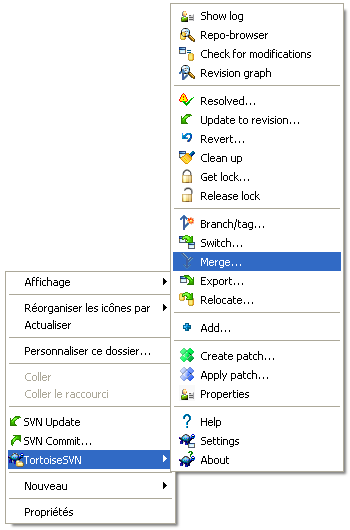
\includegraphics[width=0.50\textwidth]{mergedialog.png}
                \end{figure}
        \item Fill the form as follows.
 
		\begin{description}
		\item[From:]The first text field describes the destination, where the modifications will be made (should be the release directory in case of update of the release). You can specify from which revision you want to work. If nothing is specified, it will use the latest one.
		\item[To:] The second text field describes the source, where the reference files will be found. Typically, where SVN will find the latest version of the files (for Sofa, it will be in the trunk). You may like to use a certain revision of the file or directory; to do so, just specify a number of revision. If you don't know that number, just click on the button ``show log''. A new dialog containing all the commits, and the revision number corresponding will appear.
		\item[Diff:]Before doing the merge operation, it is practical to look at the differences that exist between your branch file/directory and the trunk one. The button ``Diff'' will do that.
		\item[Merge:] When everything is ready, just press the button ``Merge''.
		\end{description}
                \begin{figure}[htpb]
                      \centering
                                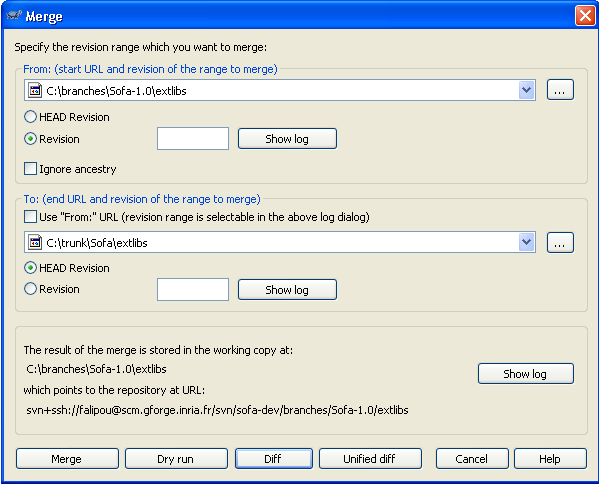
\includegraphics[width=0.90\textwidth]{mergeform.png}
                \end{figure}
		If some modifications have been done in your local branch of Sofa, you can cancel them and go back to initial state by reverting them. Right click on the file/directory, and select revert in the SVN contextual menu.
	\item Do a commit. The modification will be taken into account if only you process to a commit.
\end{itemize}
